\lab{Principal Component Analysis and Latent Semantic Indexing}{PCA and LSI}
\objective{Understand the basics of principal component analysis and latent semantic indexing.}

\section*{Principal Component Analysis}
Understanding the variance in complex data is one of the initial tasks in exploratory data analysis. For example, consider the scatter plot  displaying the sepal and petal lengths of 100 different irises shown in Figure \ref{fig:iris_1}.
\begin{figure}
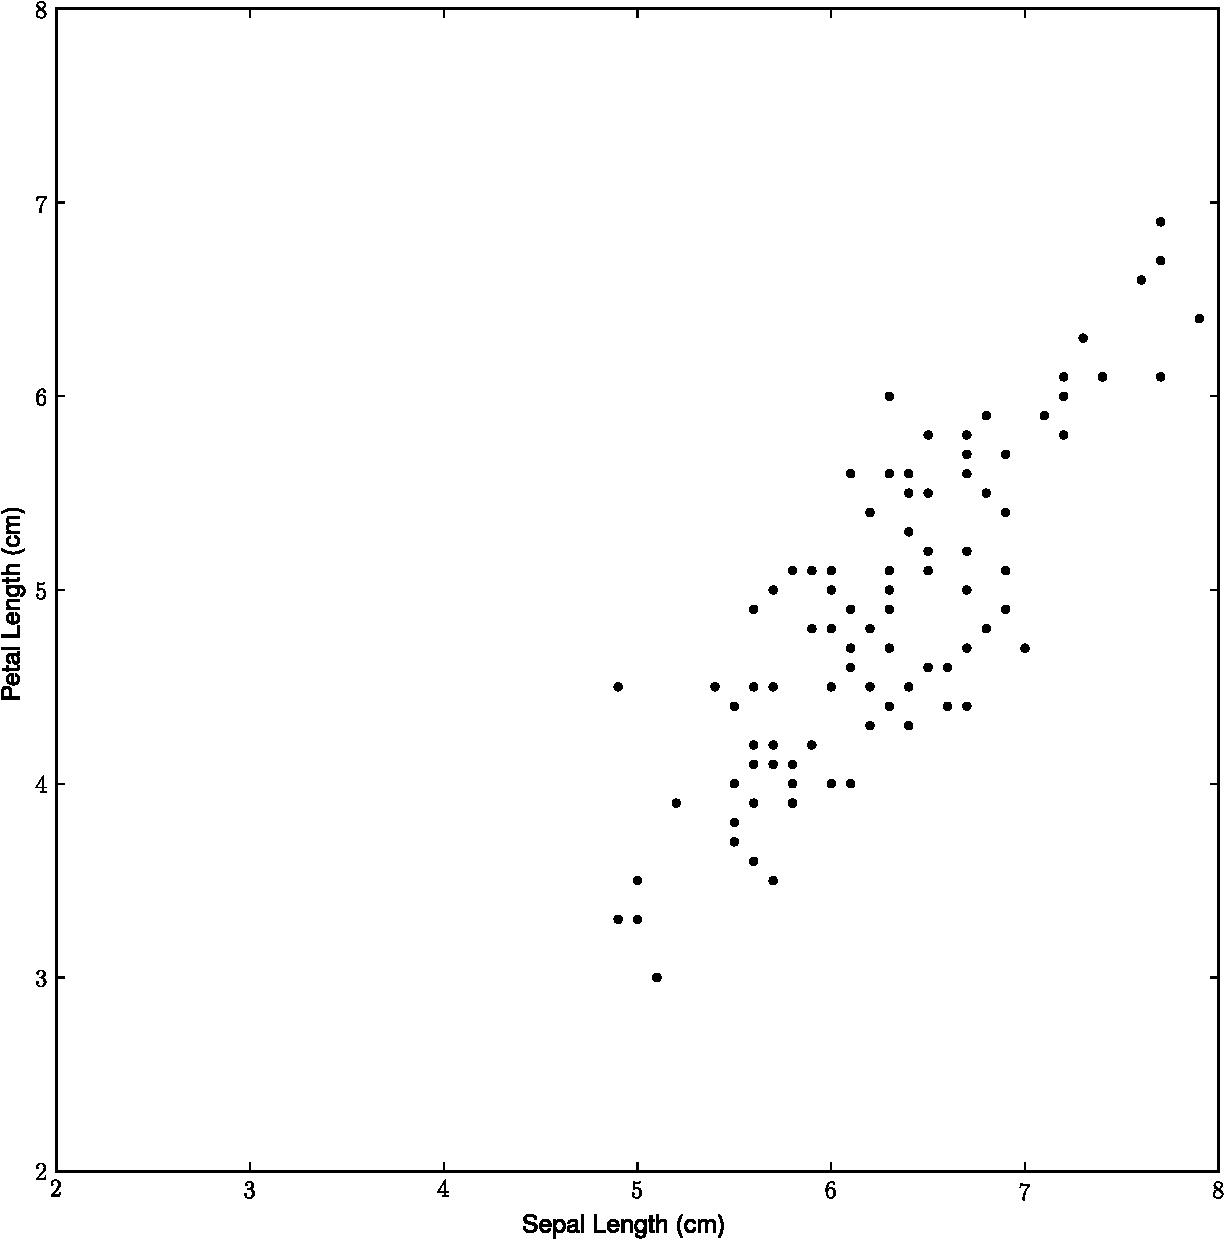
\includegraphics[width=\textwidth]{iris0.pdf}
\caption{Sepal Length vs. Petal Length for 100 iris flowers. Note the strong correlation of these variables.}
\label{fig:iris_1}
\end{figure}
There are three distinct types of iris flowers present: \emph{setosa}, \emph{versicolor}, and \emph{virginica}. 
Considering this data, we might ask how to best distinguish the different types of irises given the data about their sepal and petal lengths.
We can answer this question by finding the characteristic that causes the greatest variance in the data.
(Greater variance implies a greater ability to distinguish between data points. If the variance is very small, the data are clustered tightly together, and it is difficult to distinguish well.)

Upon examination, we see that the petal length ranges between $3$ and $7$ cm, while the sepal length only ranges between $5$ and $8$ cm. We might be tempted to say that the most distinguishing aspect of irises is their petal length, but this is only considering the features of the data individually, and not collectively. The two features of the data are clearly correlated, and a more careful consideration would lead us to conclude that the most distinguishing aspect of irises is their overall size. Some irises are are much bigger than others while the sepal and petal lengths stay roughly in proportion.
\begin{figure}
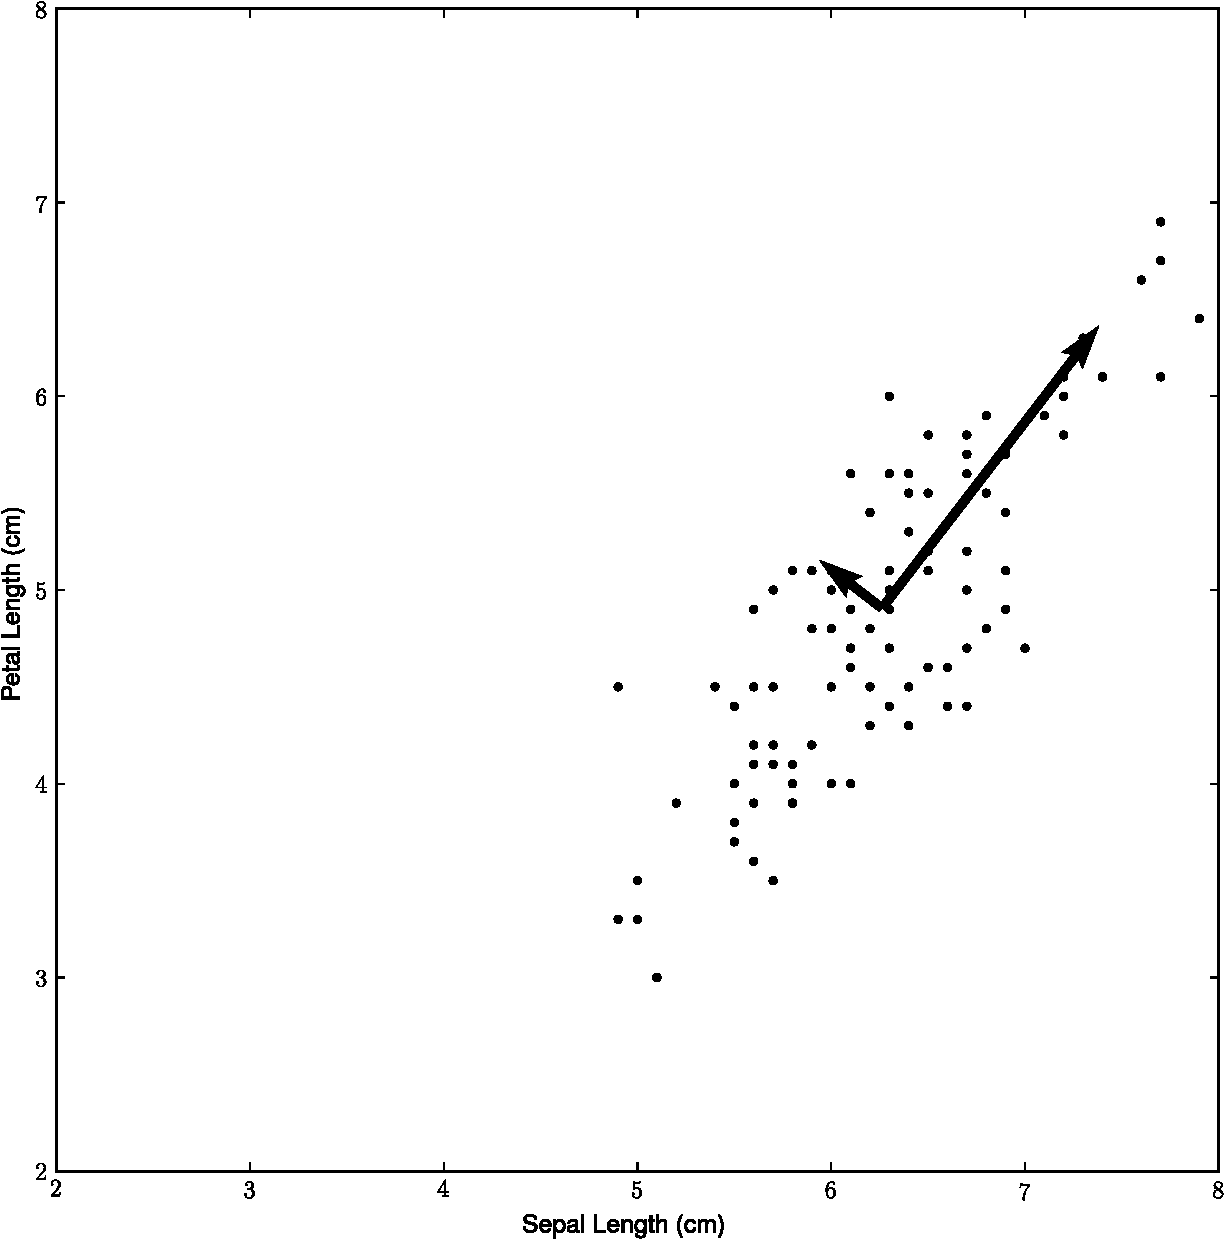
\includegraphics[width=\textwidth]{iris2.pdf}
\caption{The vectors indicate the two principal components weighted by their contribution to the variance.}
\label{fig:iris_2}
\end{figure}

Principal Component Analysis (PCA) is a multivariate statistical tool used to orthogonally change the basis of a set of observations from the basis of original features (which may be correlated) into a basis of uncorrelated (in fact, orthonormal) variables called the \emph{principal components}. It is a direct application of the singular value decomposition (SVD) from linear algebra. More specifically, the first principal component will account for the greatest variance in the set of observations, the second principal component will be orthogonal to the first, accounting for the second greatest variance in the set of observations, etc. The first several principal components capture most of the variance in the observation set, and hence provide a great deal of information about the data. By projecting the observations onto the space spanned by the principal components, we can reduce the dimensionality of the data in a manner that preserves most of the variance.

In our iris example, the two principal components are shown in Figure \ref{fig:iris_2}. The first principal component, corresponding intuitively to iris size, accounts for $96\%$ and of the variance in the data. The second, which accounts for only $4\%$ of the variance, corresponds to the relative sepal and petal length in irises of the same size.

\subsection*{Computing the Principal Components}
We now explore how to use the SVD to compute the principal components of a data set.
Throughout we will use the iris data set, which can be obtained as follows:
\begin{lstlisting}
>>> import numpy as np
>>> from scipy import linalg as la
>>> import sklearn.datasets as datasets
>>> iris = datasets.load_iris()
>>> X = iris.data
\end{lstlisting}
We represent the collection of observations as a matrix $n \times m$ matrix $X$, where each row of $X$ is an observation, and each column is a specific feature.
Let $k = \min(m,n)$. 
In the iris example, $X$ contains 150 observations, each consisting of 4 features, as shown below:
\begin{lstlisting}
>>> X.shape
(150L, 4L)
>>> iris.feature_names
['sepal length (cm)',
 'sepal width (cm)',
 'petal length (cm)',
 'petal width (cm)']
\end{lstlisting}

The first step in PCA is to pre-process the data. In particular, we first translate the columns of $X$ to have mean 0. 
The data may then be optionally scaled to remove discrepancies arising from different units of measure (i.e. centimeters vs meters), and we call the centered and scaled data $Y$.
In this lab, we will not have any scaling issues, so we won't address this further.
We pre-process our iris data as follows:
\begin{lstlisting}
>>> Y = X - X.mean(axis=0)
\end{lstlisting}

We next compute the truncated SVD of our centered and scaled data,
\[Y = U\Sigma V^{T}\]
where $U$ is $n \times k$, $\Sigma$ is a $k\times k$ diagonal matrix containing the singular values of $Y$ in decreasing order along the diagonal, and $V$ is $m \times k$. The columns of $V$ are the principal components (which form an orthonormal basis for the space spanned by the observations), and the corresponding singular values provide us information about how much variance is captured in each principal component. More specifically, let $\sigma_{i}$ be the $i$-th non-zero singular value. Then the value
\[\frac{\sigma^2_{i}}{\sum_{j=1}^{k} \sigma^2_{j}}\]
is the percentage of the variance captured by the $i$-th principal component.
We compute the truncated SVD of the iris data and show the variance percentages for each component below:
\begin{lstlisting}
>>> U,S,VT = la.svd(Y, full_matrices=False)
>>> S**2/(S**2).sum() # variance percentages
array([ 0.92461621,  0.05301557,  0.01718514,  0.00518309])
\end{lstlisting}

In general, we are only interested with the first several principal components. How many principal components exactly should we keep? There are a number of ways to decide this. One is to only keep the first two principal components, as these enable us to project the data into $2$-dimensional space, which is easy to visualize. Another way is to only keep the set of principal components accounting for a certain percentage (say $80\%$) of the variance. A third method is to examine the \emph{scree plot} of the variance percentages for each principal component, as in Figure \ref{fig:iris_scree}.
\begin{figure}
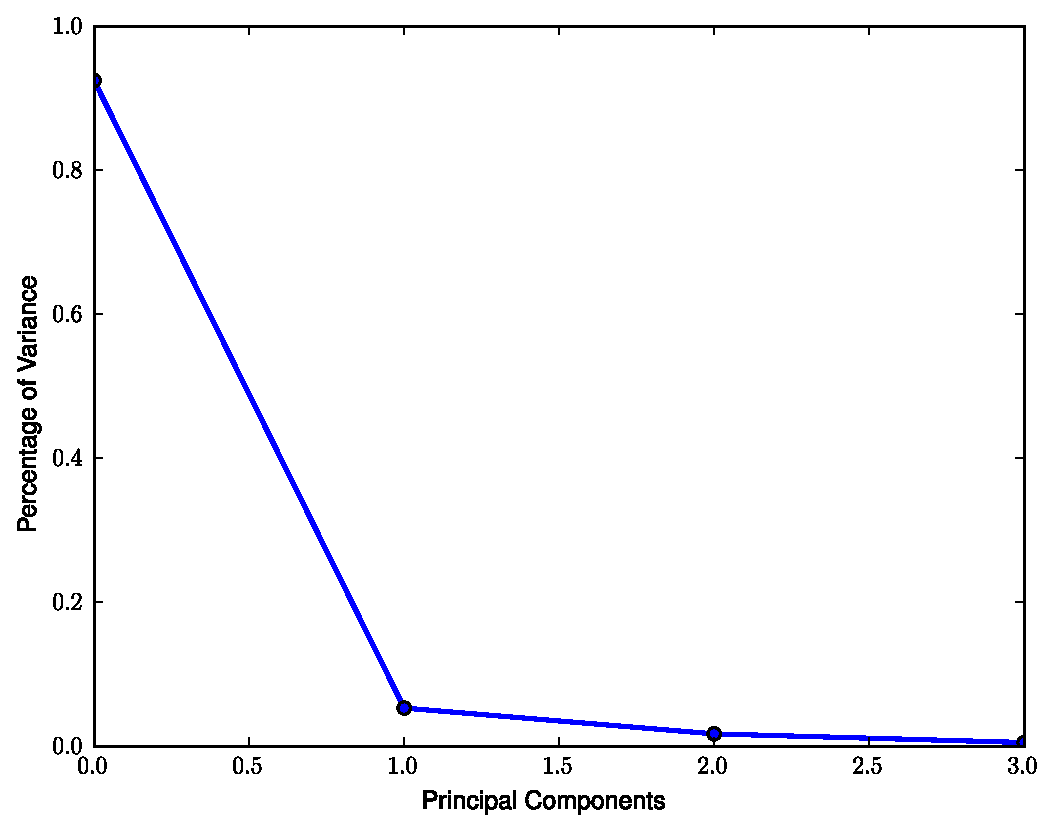
\includegraphics[width=\textwidth]{iris_scree.pdf}
\caption{Scree plot of the percentage of variance for PCA on the iris dataset.}
\label{fig:iris_scree}
\end{figure}
Upon examination of the iris scree plot, we see that there is a distinct change after the first principal component. This method is referred to as finding the ``elbow" of the scree plot, and we keep all the principal components on the left of the elbow. In the case of the iris data, that is simply the first principal component, which accounts for $92\%$ of the variance.

Once we have decided how many principal components to keep (say the first $l$), we can project the observations from the original feature space onto the principal component space by computing
\begin{equation*}
\widehat{Y} = U_l\Sigma_l
\end{equation*}
where $\Sigma_l$ is the first $l$ rows of $\Sigma$ and $U_l$ is the first $l$ columns of $U$.
Using the SVD formula, note that
\[
\widehat{Y} = YV_l,
\]
where $V_l$ is the first $l$ columns of $V$.
In this way, we see that the $i$-th row of $\widehat{Y}$ is simply the projection of the $i$-th observation onto the orthonormal set of the first $l$ principal components.
Under this projection, the data is represented in fewer dimensions, and in such a way that accentuates the variance (which can help with finding patterns within the data).

In Figure \ref{fig:iris_pca} we display the transformed iris data set, plotting the first principal component against the second. This reduction helps us to see the distinctions between the three different species, using only two dimensions instead of the full four dimensions of the feature space.
\begin{figure}
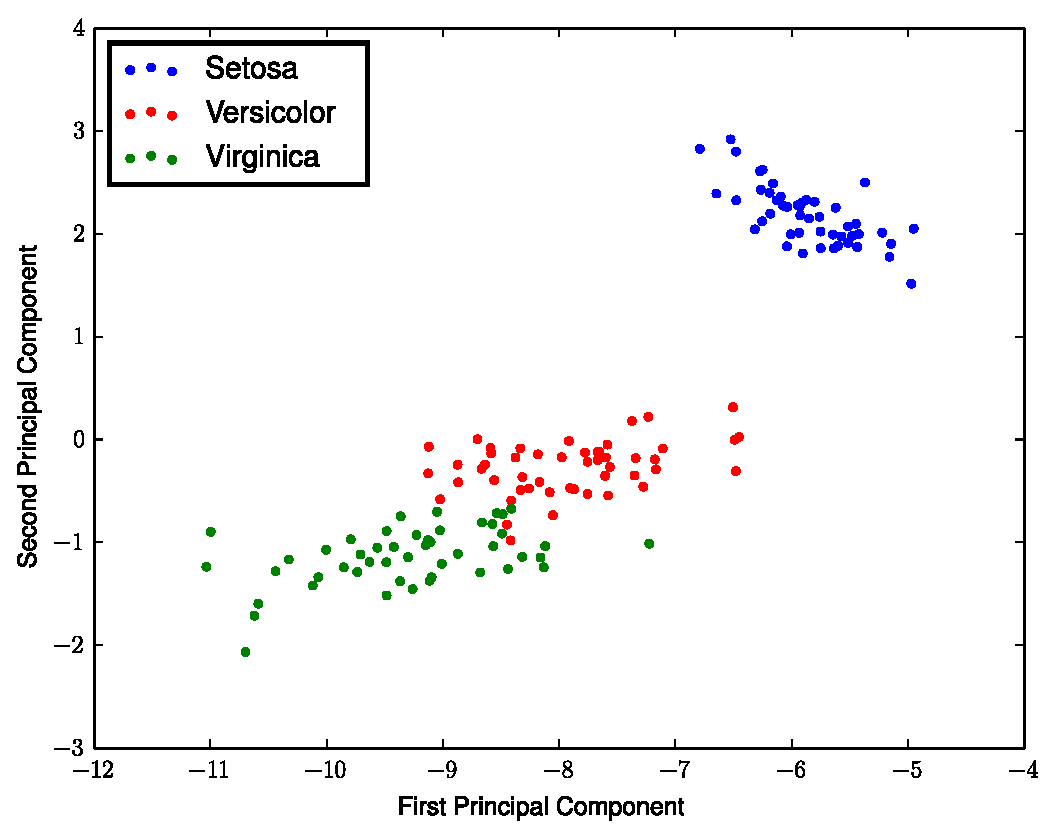
\includegraphics[width=\textwidth]{iris_pca.pdf}
\caption{Plot of transformed iris data, keeping only the first two principal components.}
\label{fig:iris_pca}
\end{figure}

\begin{problem}
Recreate the plot shown in Figure \ref{fig:iris_pca} by performing PCA on the iris dataset, keeping the first two principal components. 

\emph{Note:}
If \li{Yhat} is your $150 \times 2$ array of transformed observations, you can access the rows corresponding to the setosa flowers as follows:
\begin{lstlisting}
>>> Yhat[iris.target==0]
\end{lstlisting}
To get the rows corresponding to versicolor and virginica specimens, simply replace the $0$ with $1$ and $2$, respectively.
\end{problem}

\section*{Latent Semantic Indexing}
Let's now consider PCA in the context of natural language processing.
Suppose we have a large collection of documents. How can we find an article about PCA?
We might consider simply choosing the article that contains the acronym \emph{PCA} the greatest number of times, but this is a crude method.
A better way is to use a form of PCA on the collection of the documents.
In order to do so, we need to represent the documents as numerical vectors.
A standard way of doing this is to define an ordered set of words occurring in the collection of documents (called the \emph{vocabulary}), and then
represent each document as a vector of word counts from the vocabulary.
More formally, let our vocabulary be $V = \{w_1,w_2,\ldots,w_m\}$.
Then a document is a vector $x  = (x_1,x_2,\ldots,x_m) \in \mathbb{R}^m$ such that $x_i$ is the number of occurrences of word $w_i$ in the document.
In this setup, we represent the entire collection of $m$ documents as an $m \times n$ matrix $f$, where $m$ is the length of the vocabulary and $n$ is the number of documents in our collection, each column being a document vector. As expected, we let $f_{ij}$ be the number of times term $i$ occurs in document $j$.

We perform PCA on $f$ without centering the data so that we may retain the sparsity of $f$. We now have $f = T\Sigma D^{H}$. The $i^{th}$ row of $D$ is a vector corresponding to the $i^{th}$ document. We typically truncate these vectors, similar to identifying the important principal components of $t\!f$. We let $D_{i}$ denote the $i^{th}$ truncated row of $D$. Given a document $i$, we would like to find the document $j$ most similar to $i$, given that $i\neq j$. What we really need to compare are the vectors $D_{i}\Sigma$ and $D_{j}\Sigma$. Our metric of choice is the angle between two vectors, which is easily computable by considering the identity
\begin{equation*}
\cos \theta_{ij} = \frac{D_{i}\Sigma \cdot D_{j}\Sigma}{\|D_{i}\Sigma\| \|D_{j}\Sigma\|}
\end{equation*}
where $\theta_{ij}$ is the angle between $D_{i}\Sigma$ and $D_{j}\Sigma$. If two document vectors have a small angle between them, then they are similar; a large angle signifies that they are quite different. Since $\cos \theta_{ij}$ is large whenever $\theta_{ij}$ is small, we seek to find
\begin{equation*}
\argmax_{j} \frac{D_{i}\Sigma \cdot D_{j}\Sigma}{\|D_{i}\Sigma\| \|D_{j}\Sigma\|}
\end{equation*}
While this is the idea, in practice there are a few other steps we must take prior to the matrix decomposition. In any language, some words are so common that they provide no important information. We call these \emph{stop words}. Examples in English include \emph{the, a, an, and, I, we, you, it, there}, etc. Before processing any set of documents, we must remove all occurrences of stop words. We are going to consider the collection of all State of the Union addresses from 1945 to 2013, but these speeches are in an uncleaned format in the folder \emph{Addresses}, so we must first process them.

\begin{problem}
Using the function \li{loadStopwords} and the file
\texttt{stopwords.txt} provided, read in the stop word list in Python.
Use the functions \li{termlist}, \li{removeStopwords}, \li{uniq},
and \li{parseDocument} provided to create an array containing all of the unique
terms encountered in the corpus that are not included in the stop word list.
This is called the \emph{term list}.
\end{problem}

\begin{problem}
Write a function that accepts a file name, a list of stop words, and the term list
found above, that will return a vector whose $i^{th}$ entry is the number of
times the $i^{th}$ word from the term list occurs in the .txt file.
Note that no word in the stop word list should ever contribute to any entry of this vector.
\end{problem}

\begin{problem}
Write a function that accepts a directory, a list of stop words, and the term list,
that will make the term frequency matrix $t\!f$ as described above.
Each column in $f$ should be the value returned by the function written in the
previous problem for a particular file. In particular, $f$ should be a
$m \times n$ matrix, where $m$ is the length of the term list and
$n$ is the number of .txt files in the given directory.
\end{problem}

Not only is removing a predetermined set of stop words a good idea,
but it's also important to consider that words appearing in few documents tend
to provide more information than words occurring in every document.
For example, while the word \emph{war} might not be considered a stop word,
it is likely to appear in quite a few addresses, while \emph{Afghanistan} will not.
Thus two speeches sharing the word \emph{Afghanistan} ought to be considered more
related than two speeches sharing the word \emph{war}.
So while $f_{ij}$ is a good measure of the importance of term $i$ in document $j$,
we also need to consider some kind of global weight for each term $i$,
indicating how important the term is over the entire collection.
There are a number of different weights we could choose, but we choose to employ
the following particular approach.

Let $t_{i}$ be the total number of times term $i$ appears in the entire
collection of documents.
Define
\begin{equation*}
p_{ij} = \frac{f_{ij}}{t_{i}}
\end{equation*}
We then let
\begin{equation*}
g_{i} = 1 + \sum_{j=1}^{n} \frac{p_{ij} \log (p_{ij} + 1)}{\log n}
\end{equation*}
where $n$ is the number of documents in the collection.
We call $g_{i}$ the global weight of term $i$.
We replace each term frequency in the matrix $f$ by weighting it globally.
Specifically, we define
\begin{equation*}
a_{ij} = g_{i} \log (f_{ij} + 1)
\end{equation*}
so we can consider these values to be a matrix $A$, which will take the place of
$f$ as a matrix whose entries are both locally and globally weighted.

\begin{problem}
Write a function that accepts the term frequency matrix returned by your previous
function, and which returns the matrix $A$ as described above.
Perform PCA on $A$ as described above, remembering to \emph{not} center the data.
Truncate the document vectors to retain the first $80\%$ of the variance in the data.
\end{problem}

\begin{problem}
Write a function that accepts the truncated document matrix, the list of file names
for the documents, and an index $i$, and which returns the file name of the document
most similar to the $i^{th}$ document. Find the speeches most similar to each of
President George W. Bush's speeches, as well as the speeches most similar to
each of President Obama's speeches.
\end{problem}
